%%%%%%%%%%%%%%%%%%%%%%%%%%%%%%%%%%%%%%%%%%%%%%%%%%%%%%%%%%%%%%%%%%%%%
% LaTeX Template: Project Titlepage Modified (v 0.1) by rcx
%
% Original Source: http://www.howtotex.com
% Date: February 2014
% 
% This is a title page template which be used for articles & reports.
% 
% This is the modified version of the original Latex template from
% aforementioned website.
% 
%%%%%%%%%%%%%%%%%%%%%%%%%%%%%%%%%%%%%%%%%%%%%%%%%%%%%%%%%%%%%%%%%%%%%%

\documentclass[12pt]{report}
\usepackage[a4paper]{geometry}
\usepackage[utf8]{inputenc}
\usepackage[myheadings]{fullpage}
\usepackage{fancyhdr}
\usepackage{lastpage}
\usepackage{graphicx, wrapfig, subcaption, setspace, booktabs}
\usepackage[T1]{fontenc}
\usepackage[font=small, labelfont=bf]{caption}
\usepackage{fourier}
\usepackage[protrusion=true, expansion=true]{microtype}
\usepackage[french]{babel}
\usepackage{sectsty}
\usepackage{url, lipsum}
\usepackage{amsmath}
\usepackage{pdflscape}
\usepackage{hyperref}


% [begin] Numérotation des sections /subsec / subsubsec 
\usepackage{titlesec}
\titleformat{\chapter}
  {\Large\bfseries} % format
  {}                % label
  {0pt}             % sep
  {\huge}           % before-code

\renewcommand \thesection{\Roman{section}}
\renewcommand \thesubsection{\Roman{section}.\arabic{subsection}}
\renewcommand \thesubsubsection{\Roman{section}.\arabic{subsection}.\arabic{subsubsection}}
% [/end] Numérotation des sections /subsec / subsubsec 

% [begin] arrows with 2 heads
\usepackage{amssymb}
\usepackage{graphicx}

\newcommand\twoheaduparrow{\mathrel{\rotatebox[origin=c]{90}{$\twoheadrightarrow$}}}
% [/end]arrows with 2 heads

\onehalfspacing
\setcounter{tocdepth}{5}
\setcounter{secnumdepth}{5}




%-------------------------------------------------------------------------------
% LANGUAGES COLORATION
%-------------------------------------------------------------------------------

\usepackage{listings} 

\usepackage{color}
\usepackage[svgnames]{xcolor}
\definecolor{light-gray}{gray}{0.98}
\definecolor{gray1}{gray}{0.3}
\definecolor{dkgreen}{rgb}{0,0.6,0}
\definecolor{gray}{rgb}{0.5,0.5,0.5}
\definecolor{mauve}{rgb}{0.58,0,0.82}

%-------------------
% ASSEMBLER 68K :
%-------------------

\lstdefinelanguage
{Rule}{
basicstyle=\ttfamily
}

\lstdefinelanguage
   [68k]{Assembler}     % add a "x64" dialect of Assembler
   % with these extra keywords:
{   
   alsoletter=\#,
   identifierstyle=\idstyle, 
   keywords=[1]{LOAD, STORE, PUSH, POP, LEA, PEA, NEW, DEL, ADD, SUB, MUL, OPP, % keywords
   QUO, REM, Scc, SHL, SHR, DIV, FMA, FLOAT, INT, SETROUND_mode, BRA, Bcc, BSR, RTS, 
   RINT, RFLOAT, WINT, WFLOAT, WFLOATX, WSTR, WNL, ADDSP, SUBSP, TSTO, HALT, ERROR, 
   BOV, CMP, BEQ, BNE, BLT, BGT, BGE, BLE},
   keywordstyle=[1]\color{blue}\bfseries,
   ndkeywords=[s]{code}{,},
   ndkeywordstyle=\color{red}\bfseries,
   comment=[l]{;},
   commentstyle=\color{gray1},
   string=[s]{"}{"},
   stringstyle=\color{mauve}\ttfamily,
   keywords=[2]{R0, R1, R2, R3, R4, R5, R6, R7, R8, R9, R10, R11, R12, R13, R14, R15, R16, % GPRegisters
   GB, LB, SP},% Registers of stack   
   keywordstyle=[2]\color{dkgreen}, 
   literate={á}{{\'a}}1 {à}{{\`a}}1 {ã}{{\~a}}1 {é}{{\'e}}1 {è}{{\`e}}1 {ê}{{\^e}}1 {ç}{{\c C }}1,
   basicstyle=\ttfamily
} % etc.

\makeatletter
\newcommand*\idstyle[1]{%
         \expandafter\id@style\the\lst@token{#1}\relax%
 }
 \def\id@style#1#2\relax{%
           \ifnum\pdfstrcmp{#1}{\#}=0%
                \small\ttfamily\color{DarkRed} \the\lst@token%
            \else%
              \edef\tempa{\uccode`#1}%
              \edef\tempb{`#1}%
              \ifnum\tempa=\tempb%
                  \small\ttfamily\color{black} \the\lst@token%
              \else%
                  \the\lst@token%
             \fi%
            \fi%
 }
\makeatother

%-------------------
% JAVA :
%-------------------

\lstset{frame=tb,
  language=Java,
  aboveskip=3mm,
  belowskip=3mm,
  showstringspaces=false,
  columns=flexible,
  basicstyle={\small\ttfamily},
  numbers=none,
  numberstyle=\tiny\color{gray},
  keywordstyle=\color{blue},
  commentstyle=\color{dkgreen},
  stringstyle=\color{mauve},
  breaklines=true,
  breakatwhitespace=true,
  backgroundcolor=\color{light-gray},
  literate={á}{{\'a}}1 {à}{{\`a}}1 {ã}{{\~a}}1 {é}{{\'e}}1 {è}{{\`e}}1 {ê}{{\^e}}1 {ç}{{\c C }}1,
  tabsize=3,
  basicstyle=\ttfamily,
  linewidth=13.3cm,
  %xleftmargin=0cm,
  %xrightmargin=-3.3cm,
}
\usepackage[indent]{caption}
\setcaptionwidth{0.6\textwidth} %largeur de la légende
\setlength{\captionmargin}{10cm}
%-------------------------------------------------------------------------------
% HEADER & FOOTER
%-------------------------------------------------------------------------------
\pagestyle{fancy}
\fancyhf{}
\setlength\headheight{15pt}
\fancyhead[L]{Gl 10}                     % Group number
\fancyhead[C]{Documentation Utilisateur} % Title of the document
\fancyhead[R]{Projet Génie Logiciel}     % Course name
\fancyfoot[R]{Page \thepage\ of \pageref{LastPage}}
%-------------------------------------------------------------------------------
% TITLE PAGE
%-------------------------------------------------------------------------------

\begin{document}


\begin{titlepage}

\newcommand{\quotes}[1]{``#1''}

\newcommand{\HRule}{\rule{\linewidth}{0.5mm}} % Defines a new command for the horizontal lines, change thickness here
 
%----------------------------------------------------------------------------------------
%	HEADING SECTIONS
%----------------------------------------------------------------------------------------
% Logo of the University :
$~~$
\\[-3cm]

\includegraphics[width=0.35\textwidth]{./ressources/logo-ensimag.jpg}\\ [2cm]

\center % Center everything on the page
\textsc{\LARGE Projet CAWEB / ACVL}\\[0.5cm] % Major heading such as course name
\textsc{\Large $2^{e}$ année}\\[1.5cm] % Minor heading such as course title


%----------------------------------------------------------------------------------------
%	TITLE SECTION
%----------------------------------------------------------------------------------------

\HRule \\[0.8cm]
{ \huge \bfseries Documentation}\\[0.4cm] % Title of your document
\HRule \\[1.0cm]
 
%----------------------------------------------------------------------------------------
%	AUTHOR SECTION
%----------------------------------------------------------------------------------------

\begin{minipage}{0.4\textwidth}
\begin{flushleft} \large
\emph{Groupe:}\\
Equipe 10 \\[0.8cm]
\emph{Auteurs:}\\
Raphael \textsc{LAGUERRE},\\ Florian \textsc{PERROUD},\\ Alexandre \textsc{RUPP}\\% Your name
\end{flushleft}
\end{minipage}
~
\begin{minipage}{0.4\textwidth}
\begin{flushright} \large
\emph{Enseignant responsable :} \\
 Nils \textsc{Gesbert} % Supervisor's Name
\end{flushright}
\end{minipage}\\[3cm]

% If you don't want a supervisor, uncomment the two lines below and remove the section above
%\Large \emph{Author:}\\
%John \textsc{Smith}\\[3cm] % Your name

%----------------------------------------------------------------------------------------
%	DATE SECTION
%----------------------------------------------------------------------------------------
{\Large Grenoble INP - Ensimag}\\[0.8cm]
{\large \today}\\[3cm] % Date, change the \today to a set date if you want to be precise

%----------------------------------------------------------------------------------------
%	LOGO SECTION
%----------------------------------------------------------------------------------------

%\includegraphics{Logo}\\[1cm] % Include a department/university logo - this will require the graphicx package
 
%----------------------------------------------------------------------------------------

\vfill % Fill the rest of the page with whitespace

\end{titlepage}


%\maketitle
\tableofcontents
\newpage

%-------------------------------------------------------------------------------
% Section title formatting
\sectionfont{\scshape}
%-------------------------------------------------------------------------------

%-------------------------------------------------------------------------------
% TOOLS (samples to copy/paste)
%-------------------------------------------------------------------------------

% for pictures : 

%\begin{figure}[!h]
%\centering
%\section{Conception Entité/Association~~~~~~~~~~~~~~~~~~~~}
%\includegraphics[height=1.95\textwidth]{../uml/BDD_schema.pdf}
%\caption{Schéma Entité/Association UML.}
%\end{figure}


%-------------------------------------------------------------------------------
% BODY
%-------------------------------------------------------------------------------

% ------------------------------------------------------------------------------
% ------------------------------ ANALYSE ---------------------------------------
% ------------------------------------------------------------------------------
\section{Analyse}

\subsection{Acteurs}
Nous avons identifié les acteurs suivants :
\begin{itemize}
\item Visiteur
\item Consommateur
\item Producteur
\item Responsable de planning
\end{itemize}
\clearpage


\begin{figure}[!h]
\centering
\subsection{Diagramme de cas d'utilisations~~~~~~~~~~~~~~~~~~~~~~~~~~~~~~~}
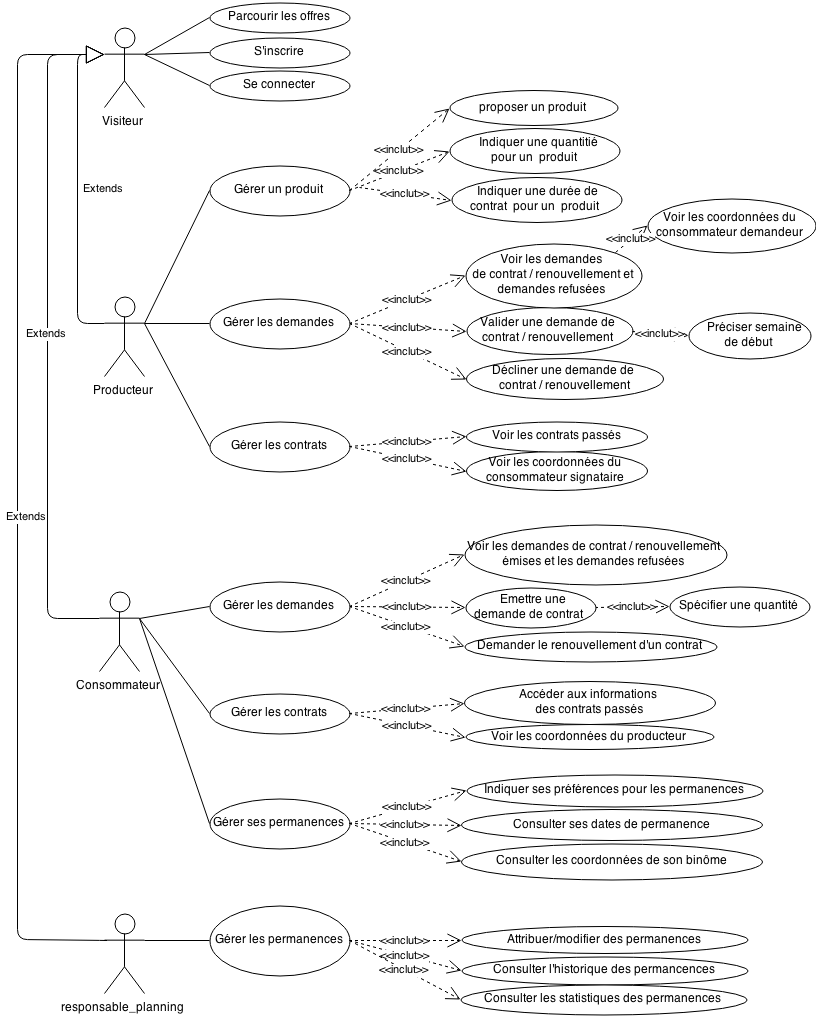
\includegraphics[height=1.35\textwidth]{./ressources/use_case.png}
\caption{Diagramme de cas d'utilisation.}
\end{figure}
\clearpage

\subsection{Description des cas d'utilisations et diagrammes de séquence système}

\subsubsection{Cas du visiteur :}

\begin{figure}[!h]
\centering
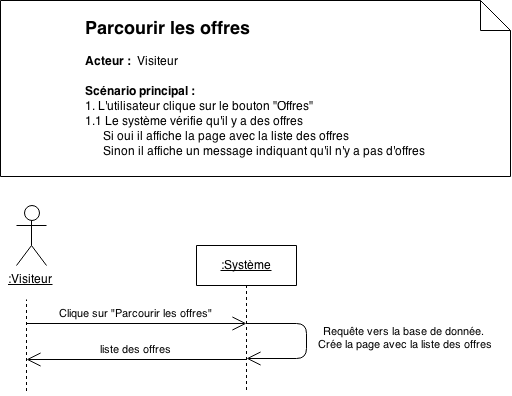
\includegraphics[width=1.\textwidth]{./ressources/desc_UC_parcourir_offres.png}
\caption{Description du cas "parcourir les offres"}
\end{figure}
\clearpage

\begin{figure}[!h]
\centering
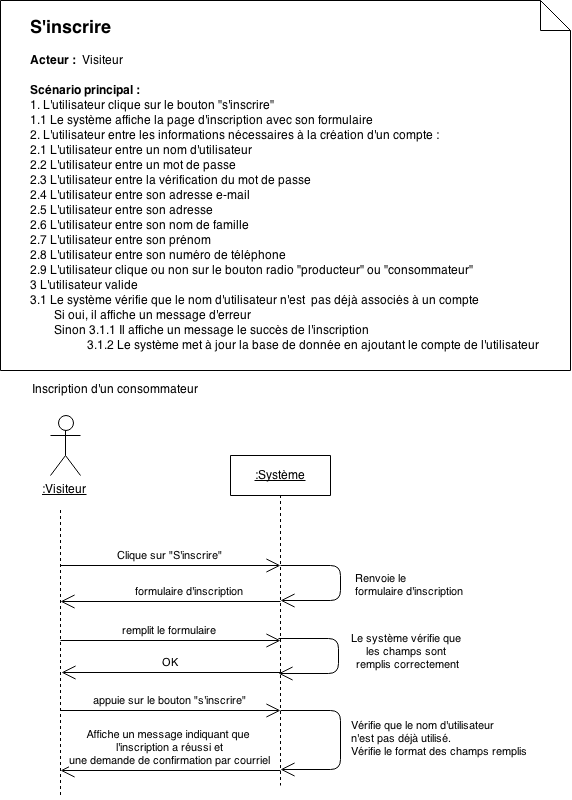
\includegraphics[width=1.\textwidth]{./ressources/desc_UC_inscrire.png}
\caption{Description du cas "s'inscrire"}
\end{figure}

\begin{figure}[!h]
\centering
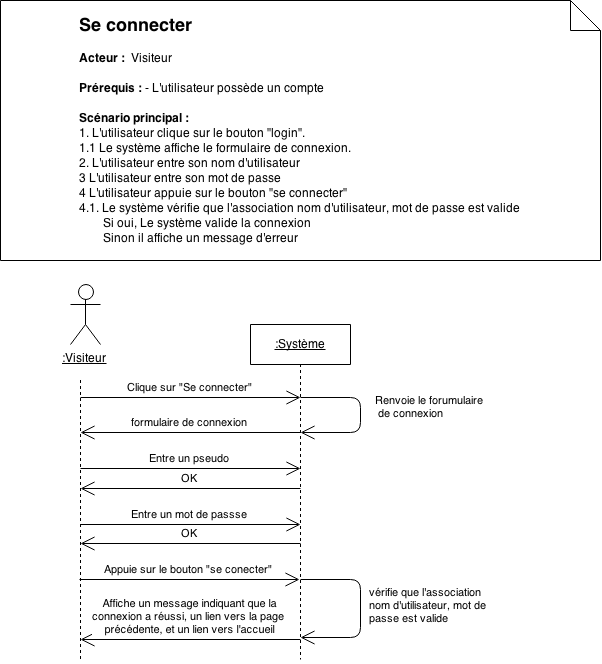
\includegraphics[width=1.\textwidth]{./ressources/desc_UC_connecter.png}
\caption{Description du cas "se connecter"}
\end{figure}
\clearpage

\subsubsection{Cas du producteur :}
\paragraph*{Gestion des produits :}
\begin{figure}[!h]
\centering
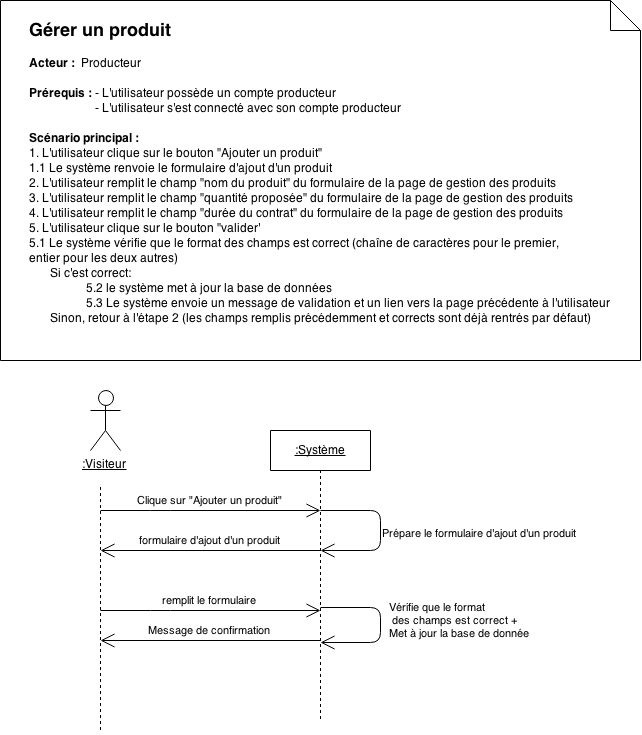
\includegraphics[width=1.\textwidth]{./ressources/desc_UC_gerer_produit.png}
\caption{Description du cas "gérer les produits"}
\end{figure}
\clearpage

\paragraph*{Gestion des demandes :}
\begin{figure}[!h]
\centering
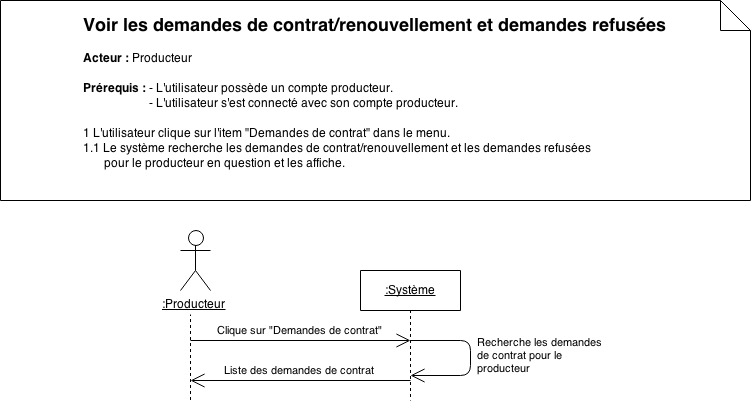
\includegraphics[width=1.\textwidth]{./ressources/desc_UC_voir_demandes_prod.png}
\caption{Description du cas "Voir les demandes de contrats/renouvellement et demandes refusées (producteur)"}
\end{figure}
\clearpage

\begin{figure}[!h]
\centering
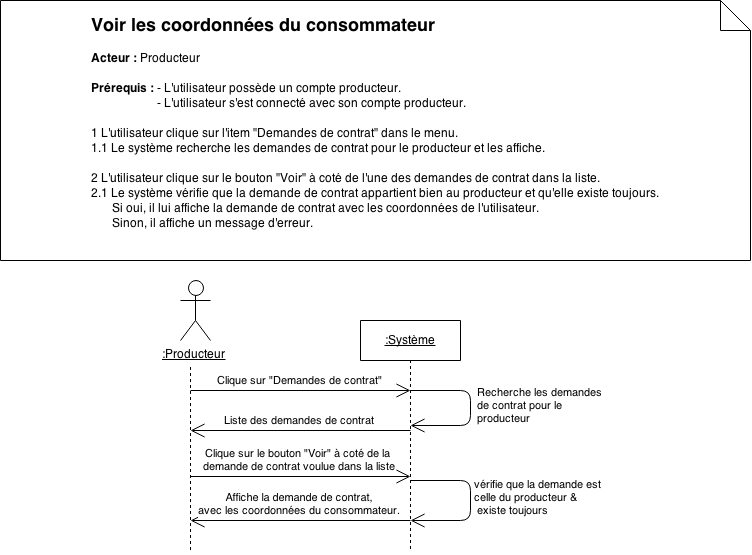
\includegraphics[width=1.\textwidth]{./ressources/desc_UC_coo_user.png}
\caption{Description du cas "Voir les coordonnées de l'utilisateur"}
\end{figure}
\clearpage

\begin{figure}[!h]
\centering
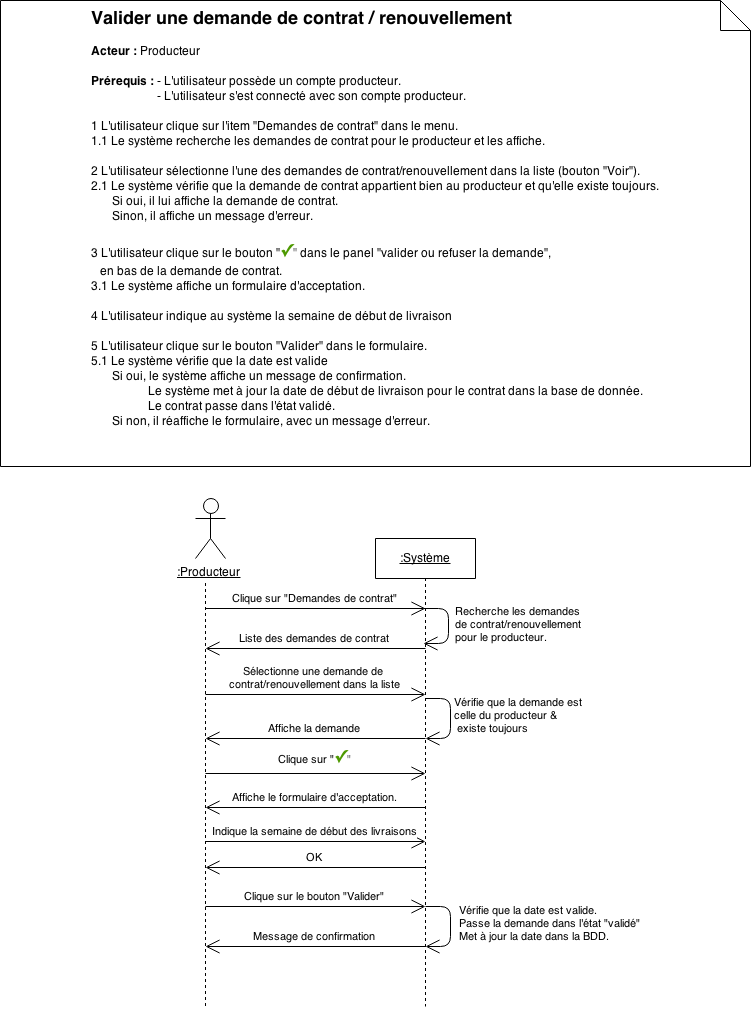
\includegraphics[width=1.\textwidth]{./ressources/desc_UC_valider_demande.png}
\caption{Description du cas "Valider une demande"}
\end{figure}
\clearpage

\begin{figure}[!h]
\centering
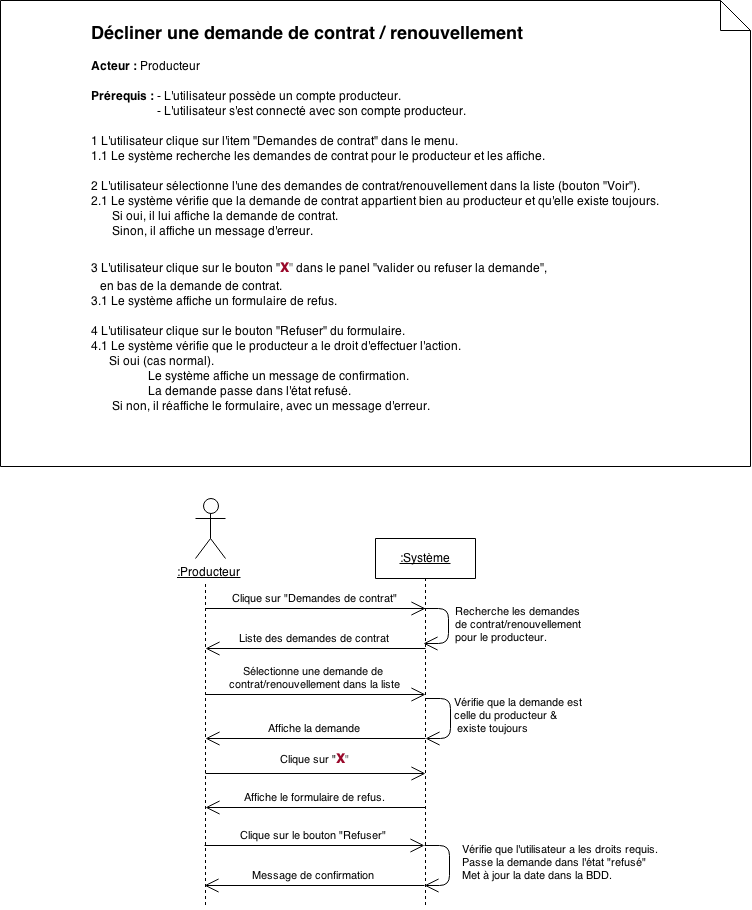
\includegraphics[width=1.\textwidth]{./ressources/desc_UC_decliner_demande.png}
\caption{Description du cas "Décliner une demande"}
\end{figure}
\clearpage

\paragraph*{Gestion des contrats :}

\begin{figure}[!h]
\centering
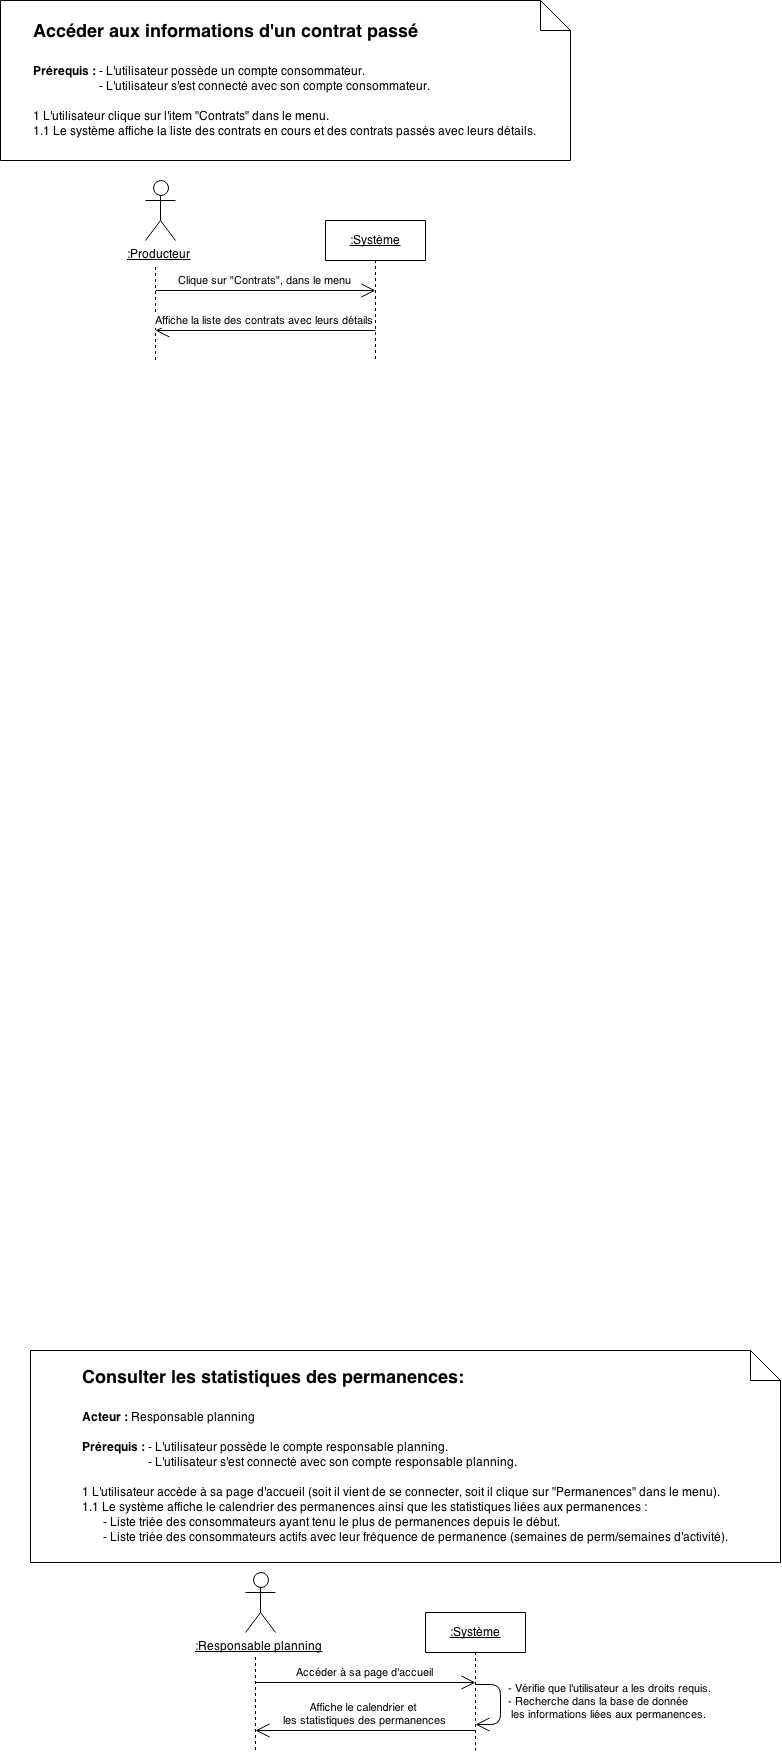
\includegraphics[width=1.\textwidth]{./ressources/desc_UC_contrats_passes.png}
\caption{Description du cas "Accéder aux informations des contrats passé (producteur)"}
\end{figure}
\clearpage

\begin{figure}[!h]
\centering
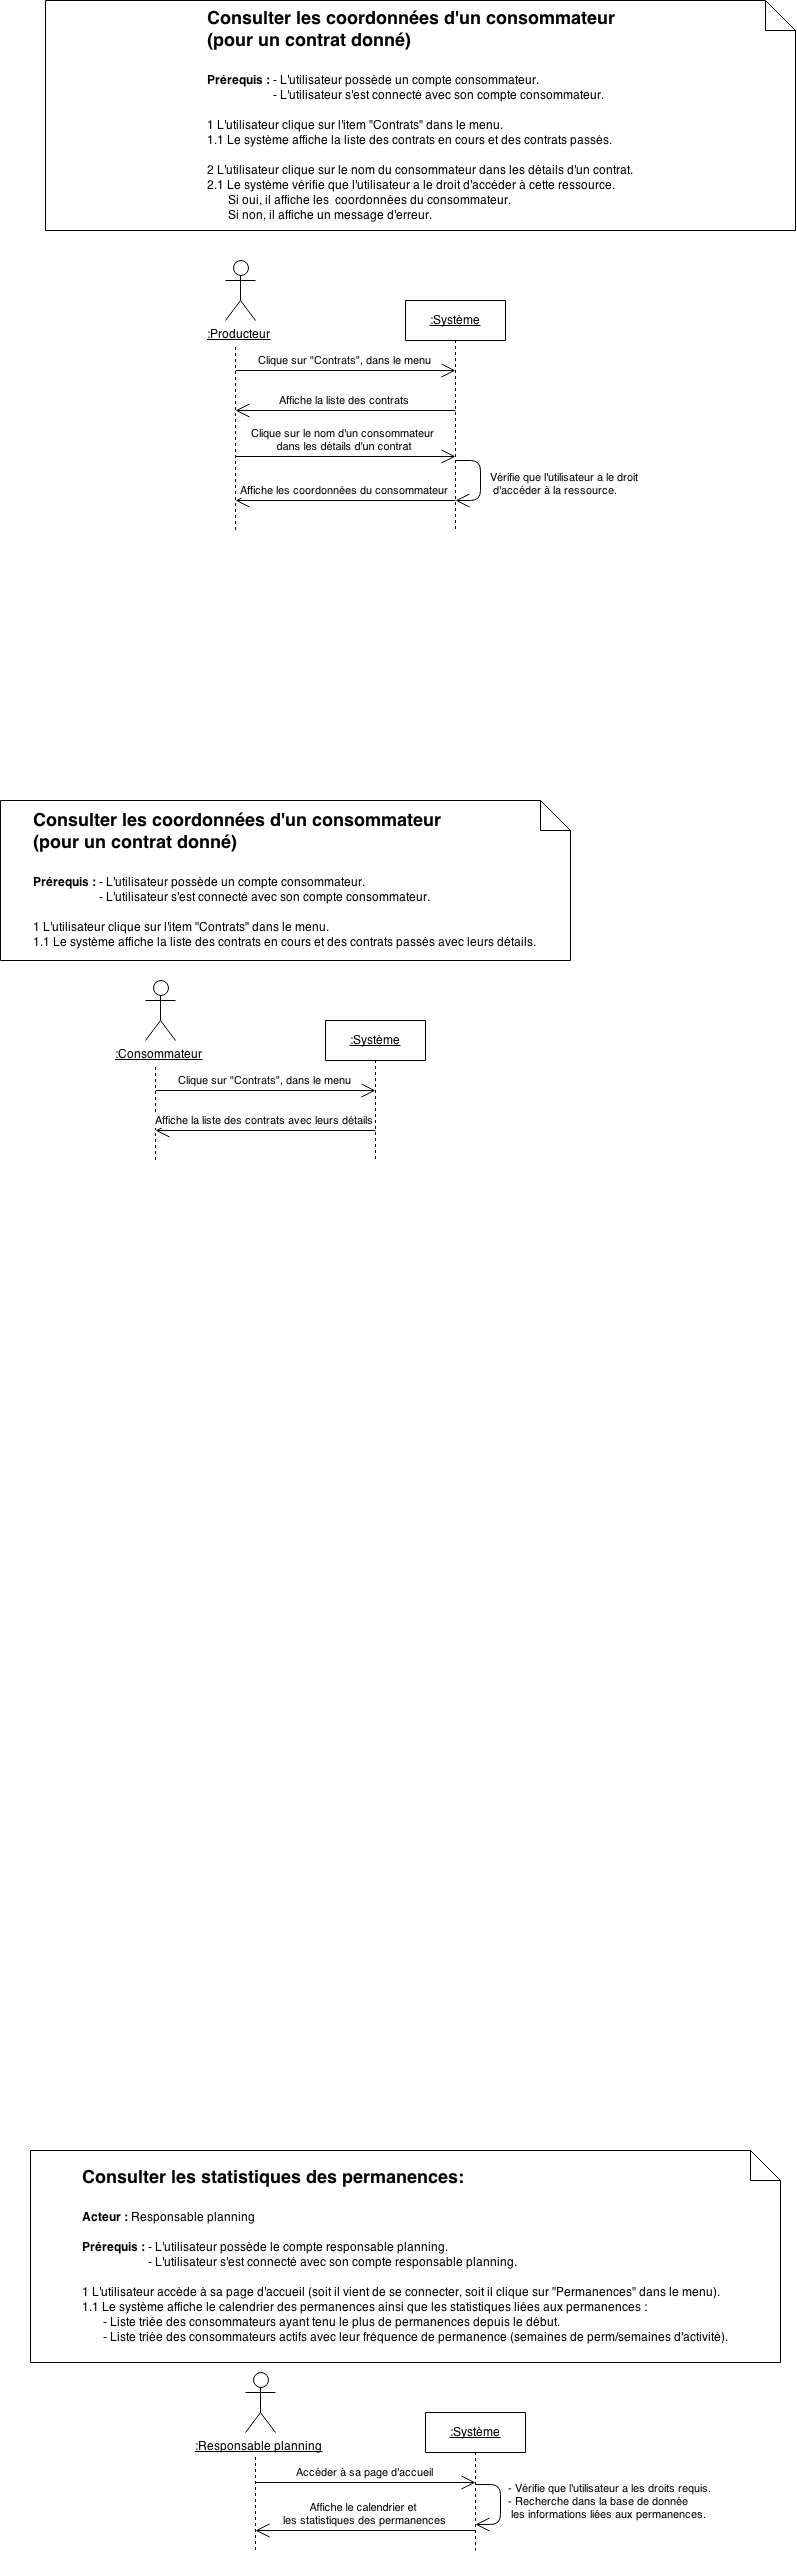
\includegraphics[width=1.\textwidth]{./ressources/desc_UC_coo_conso_contrats.png}
\caption{Description du cas "Consulter les coordonnées du consommateur signataire"}
\end{figure}
\clearpage



\subsubsection{Cas du consommateur :}
\paragraph*{Gestion des demandes :}

\begin{figure}[!h]
\centering
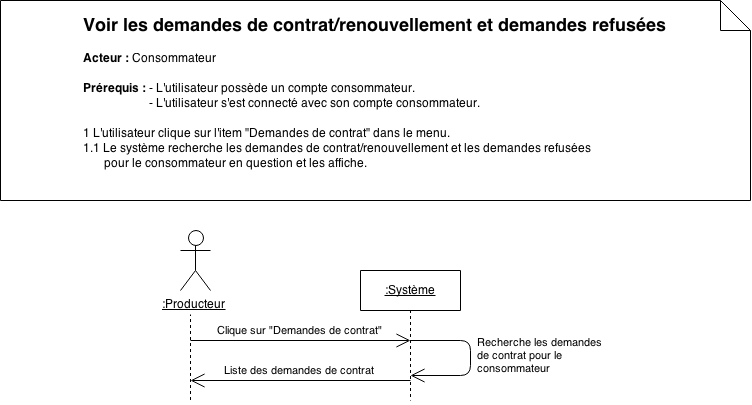
\includegraphics[width=1.\textwidth]{./ressources/desc_UC_voir_demandes_cons.png}
\caption{Description du cas "Voir les demandes de contrats/renouvellement et demandes refusées (consommateur)"}
\end{figure}
\clearpage

\begin{figure}[!h]
\centering
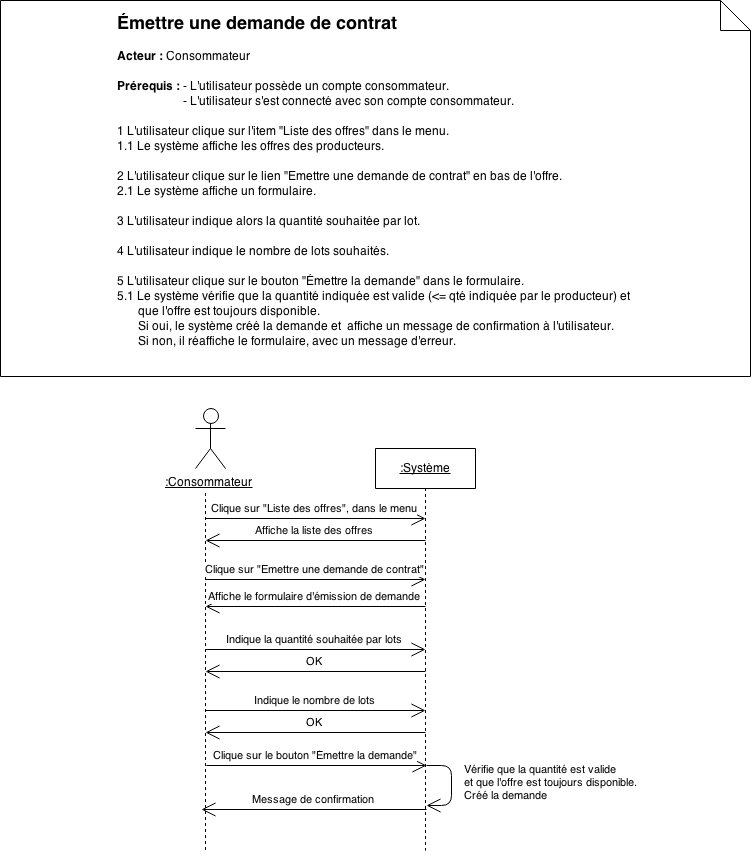
\includegraphics[width=1.\textwidth]{./ressources/desc_UC_emettre_demande.png}
\caption{Description du cas "Emettre une demande de contrat"}
\end{figure}
\clearpage

\begin{figure}[!h]
\centering
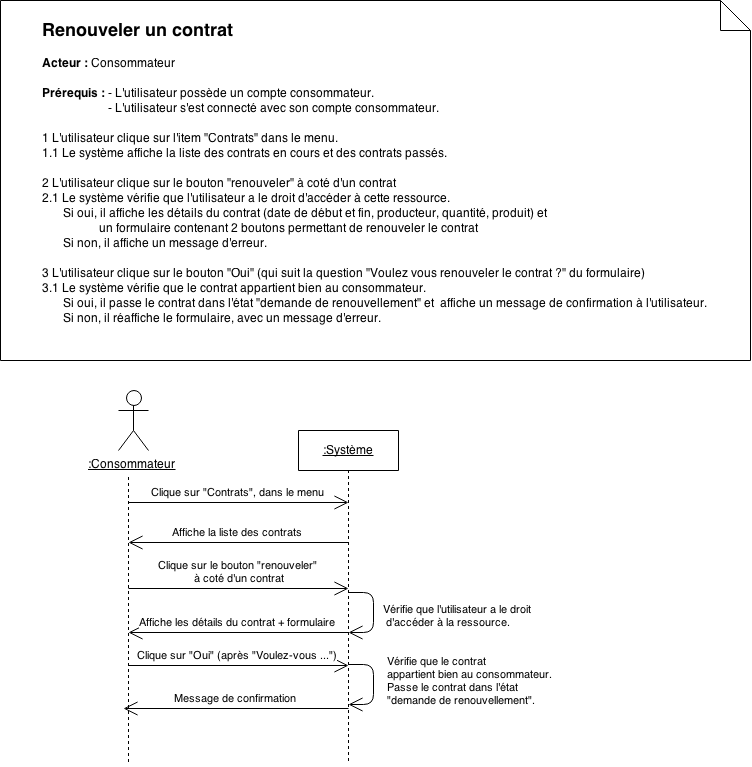
\includegraphics[width=1.\textwidth]{./ressources/desc_UC_demander_renouvellement.png}
\caption{Description du cas "Demander le renouvellement d'un contrat"}
\end{figure}
\clearpage

\paragraph*{Gestion des contrats :}
\begin{figure}[!h]
\centering
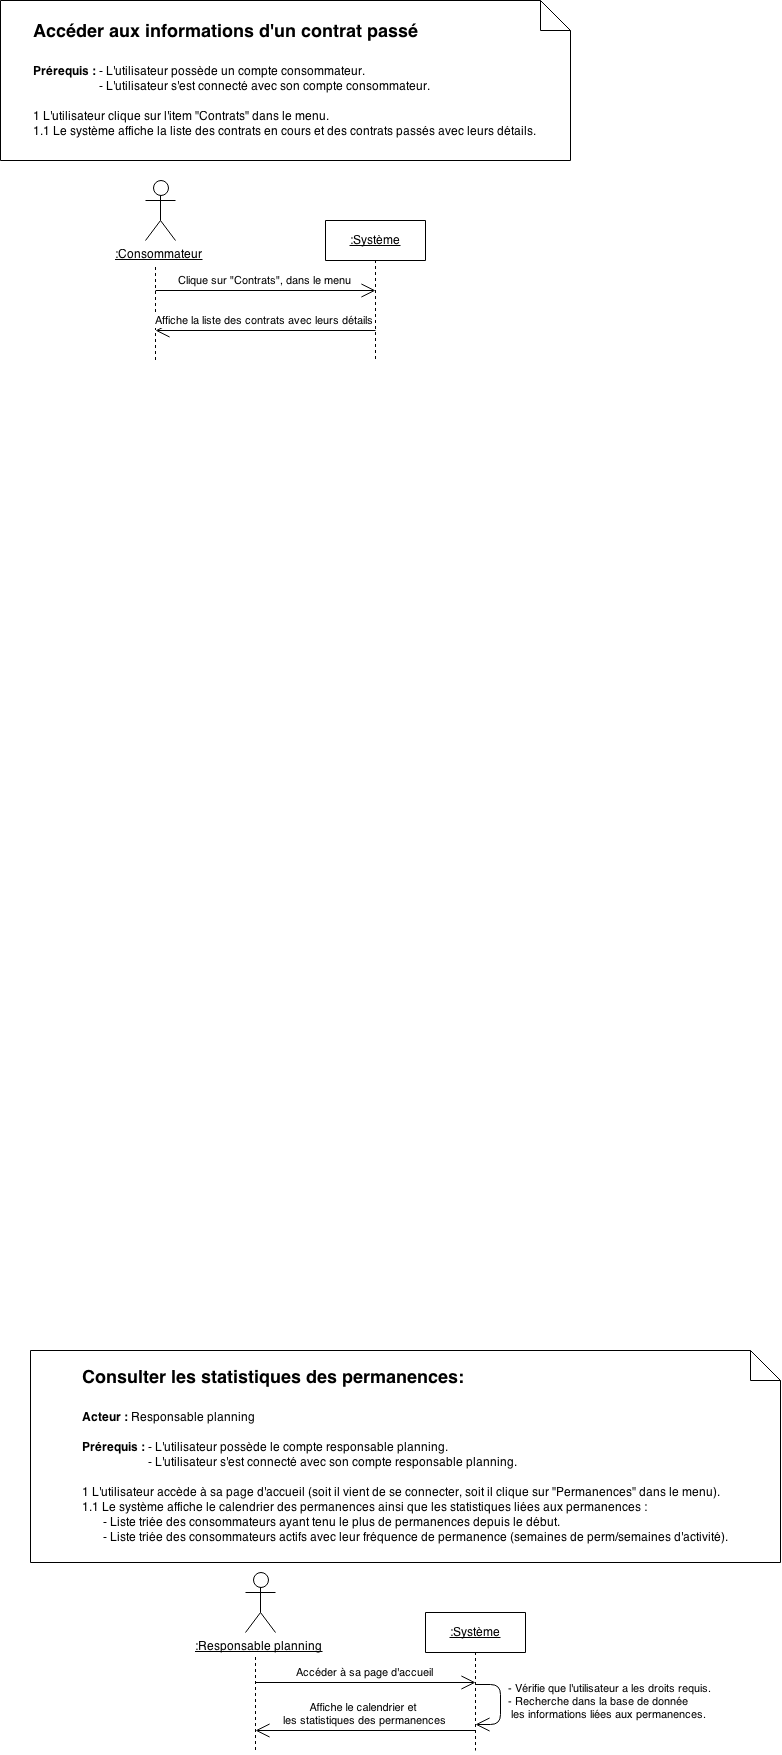
\includegraphics[width=1.\textwidth]{./ressources/desc_UC_contrats_passes_conso.png}
\caption{Description du cas "Accéder aux informations des contrats passés (consommateur)"}
\end{figure}
\clearpage

\begin{figure}[!h]
\centering
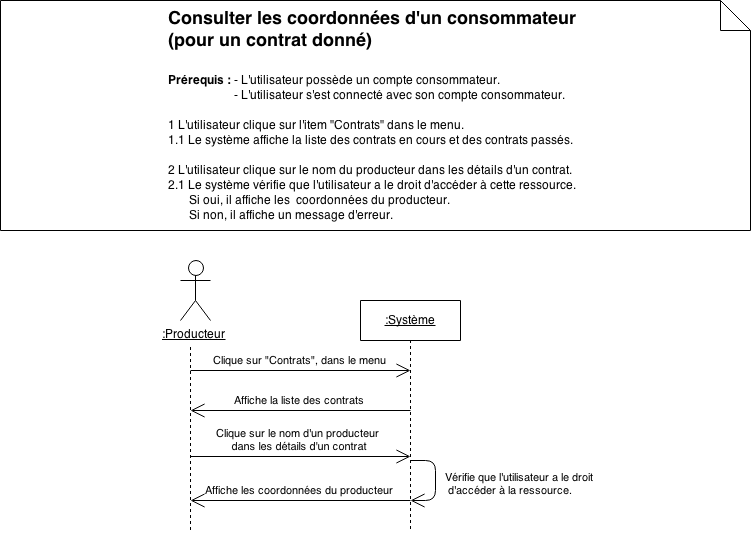
\includegraphics[width=1.\textwidth]{./ressources/desc_UC_coo_prod_contrats.png}
\caption{Description du cas "Consulter les coordonnées d'un producteur"}
\end{figure}
\clearpage


\paragraph*{Gestion des permanences :}

\begin{figure}[!h]
\centering
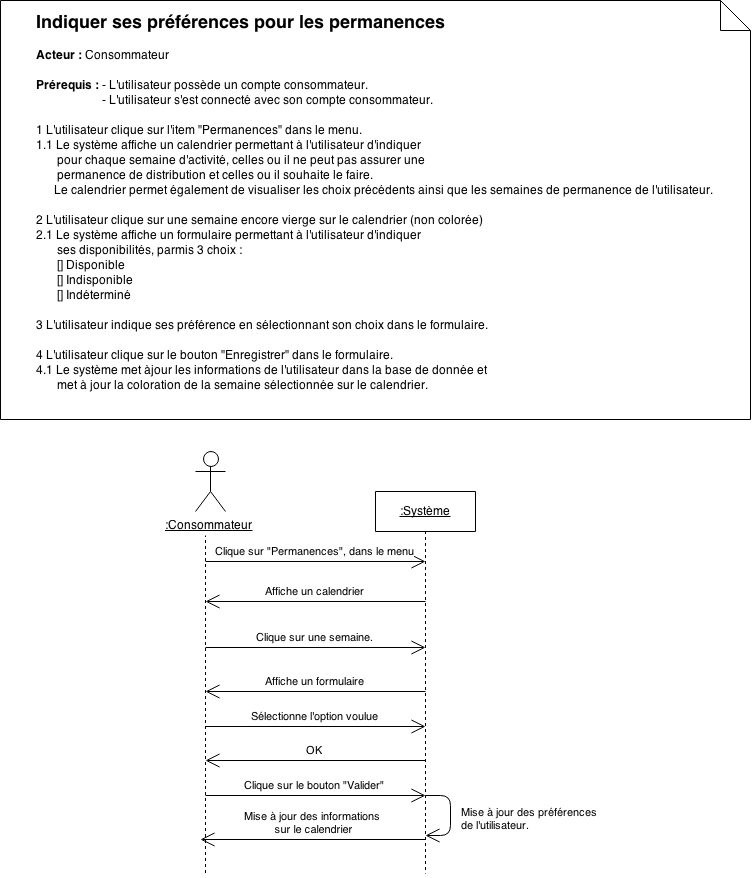
\includegraphics[width=1.\textwidth]{./ressources/desc_UC_preferences_calendrier.png}
\caption{Description du cas "Indiquer ses préférences concernant les permanences"}
\end{figure}
\clearpage

\begin{figure}[!h]
\centering
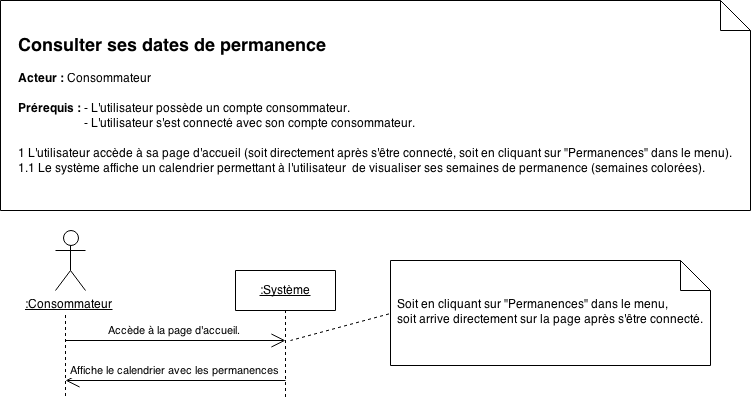
\includegraphics[width=1.\textwidth]{./ressources/desc_UC_consulter_permanences.png}
\caption{Description du cas "Consulter ses dates de permanence"}
\end{figure}
\clearpage

\begin{figure}[!h]
\centering
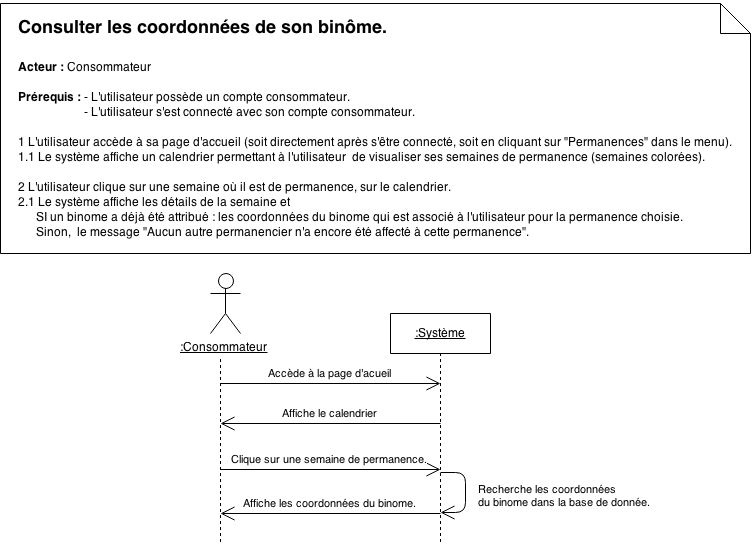
\includegraphics[width=1.\textwidth]{./ressources/desc_UC_coo_binome.png}
\caption{Description du cas "Consulter les coordonées de son binôme"}
\end{figure}
\clearpage

\subsubsection{Cas du responsable planning :}
\paragraph*{Gestion des permanences}
\begin{figure}[!h]
\centering
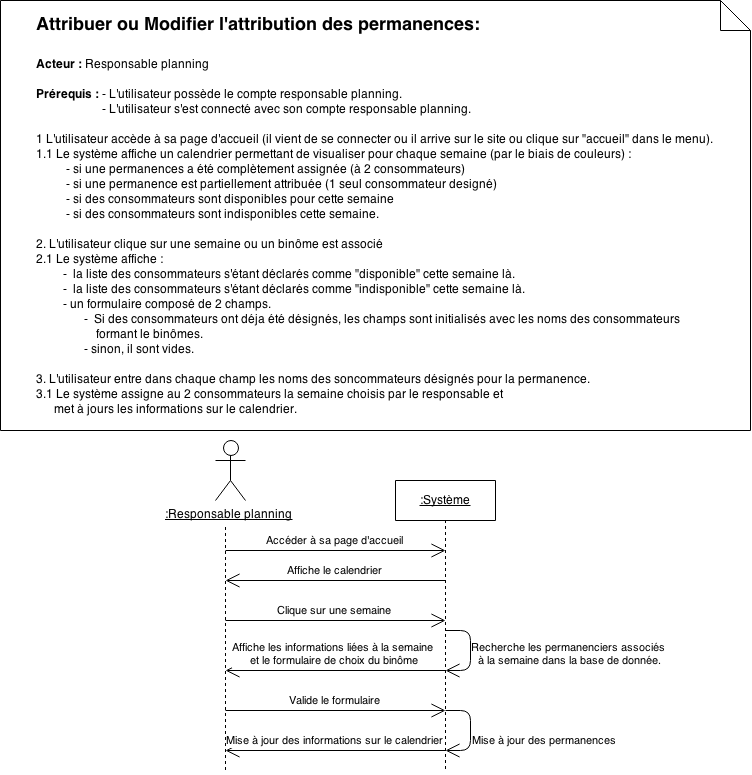
\includegraphics[width=1.\textwidth]{./ressources/desc_UC_attribuer_permanences.png}
\caption{Description du cas "Attribuer ou modifier l'attribution des permanences"}
\end{figure}
\clearpage

\begin{figure}[!h]
\centering
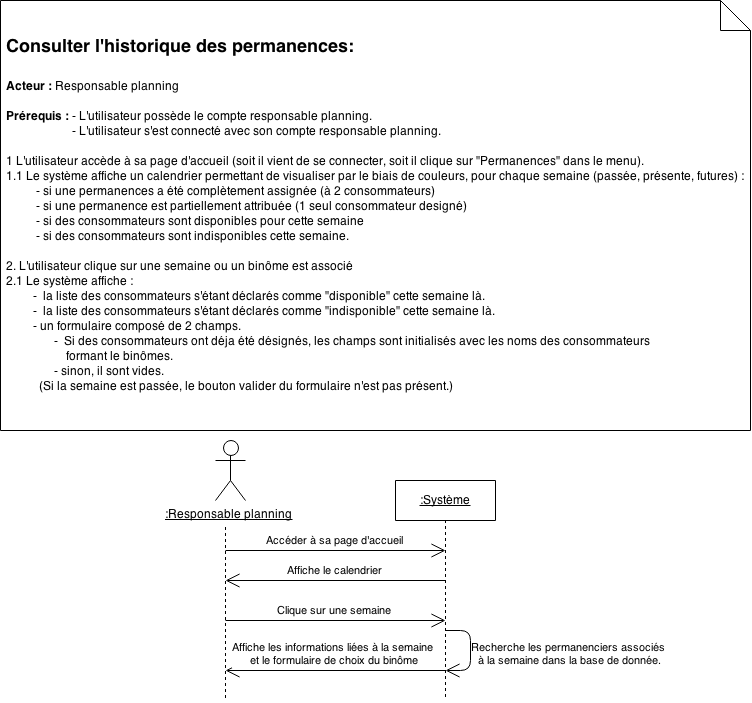
\includegraphics[width=1.\textwidth]{./ressources/desc_UC_voir_permanences.png}
\caption{Description du cas "Consulter l'historique des permanences"}
\end{figure}
\clearpage

\begin{figure}[!h]
\centering
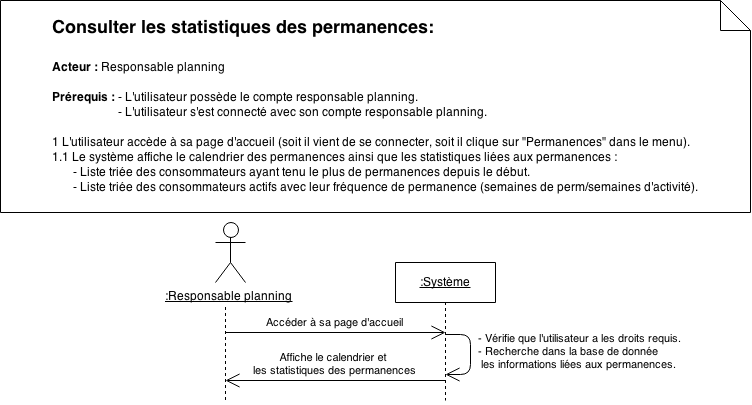
\includegraphics[width=1.\textwidth]{./ressources/desc_UC_stats_permanences.png}
\caption{Description du cas "Consulter les statistiques des permanences"}
\end{figure}
\clearpage




\clearpage

\begin{figure}[!h]
\centering
\subsection{Diagramme de classes d'analyse~~~~~~~~~~~~~~~~~~~~~~~~~~~~~~~}
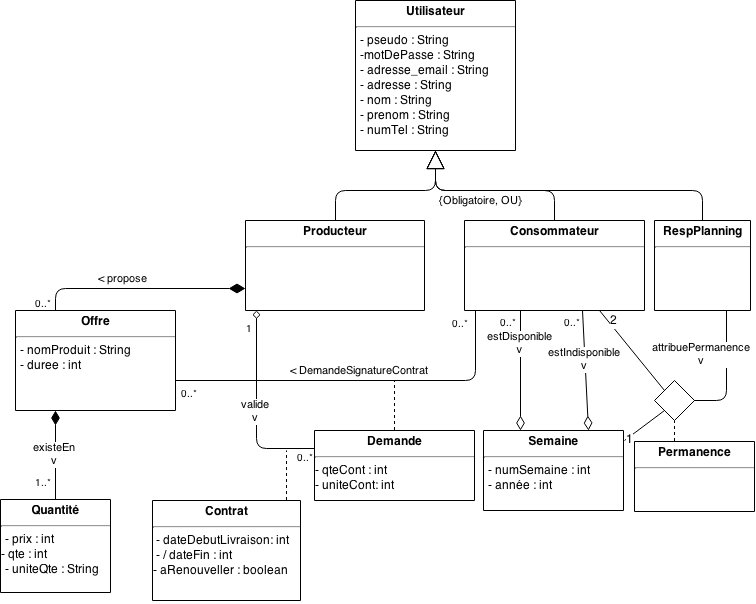
\includegraphics[height=.9\textwidth]{./ressources/class_analyse.png}
\caption{Diagramme de classes d'analyse.}
\end{figure}
\clearpage

% ------------------------------------------------------------------------------
% --------------------------- CONCEPTION ---------------------------------------
% ------------------------------------------------------------------------------

\section{Conception}

\begin{figure}[!hp]
\centering
\subsection{Architecture générale~~~~~~~~~~~~~~~~~~~~~~~~~~~~~~~}
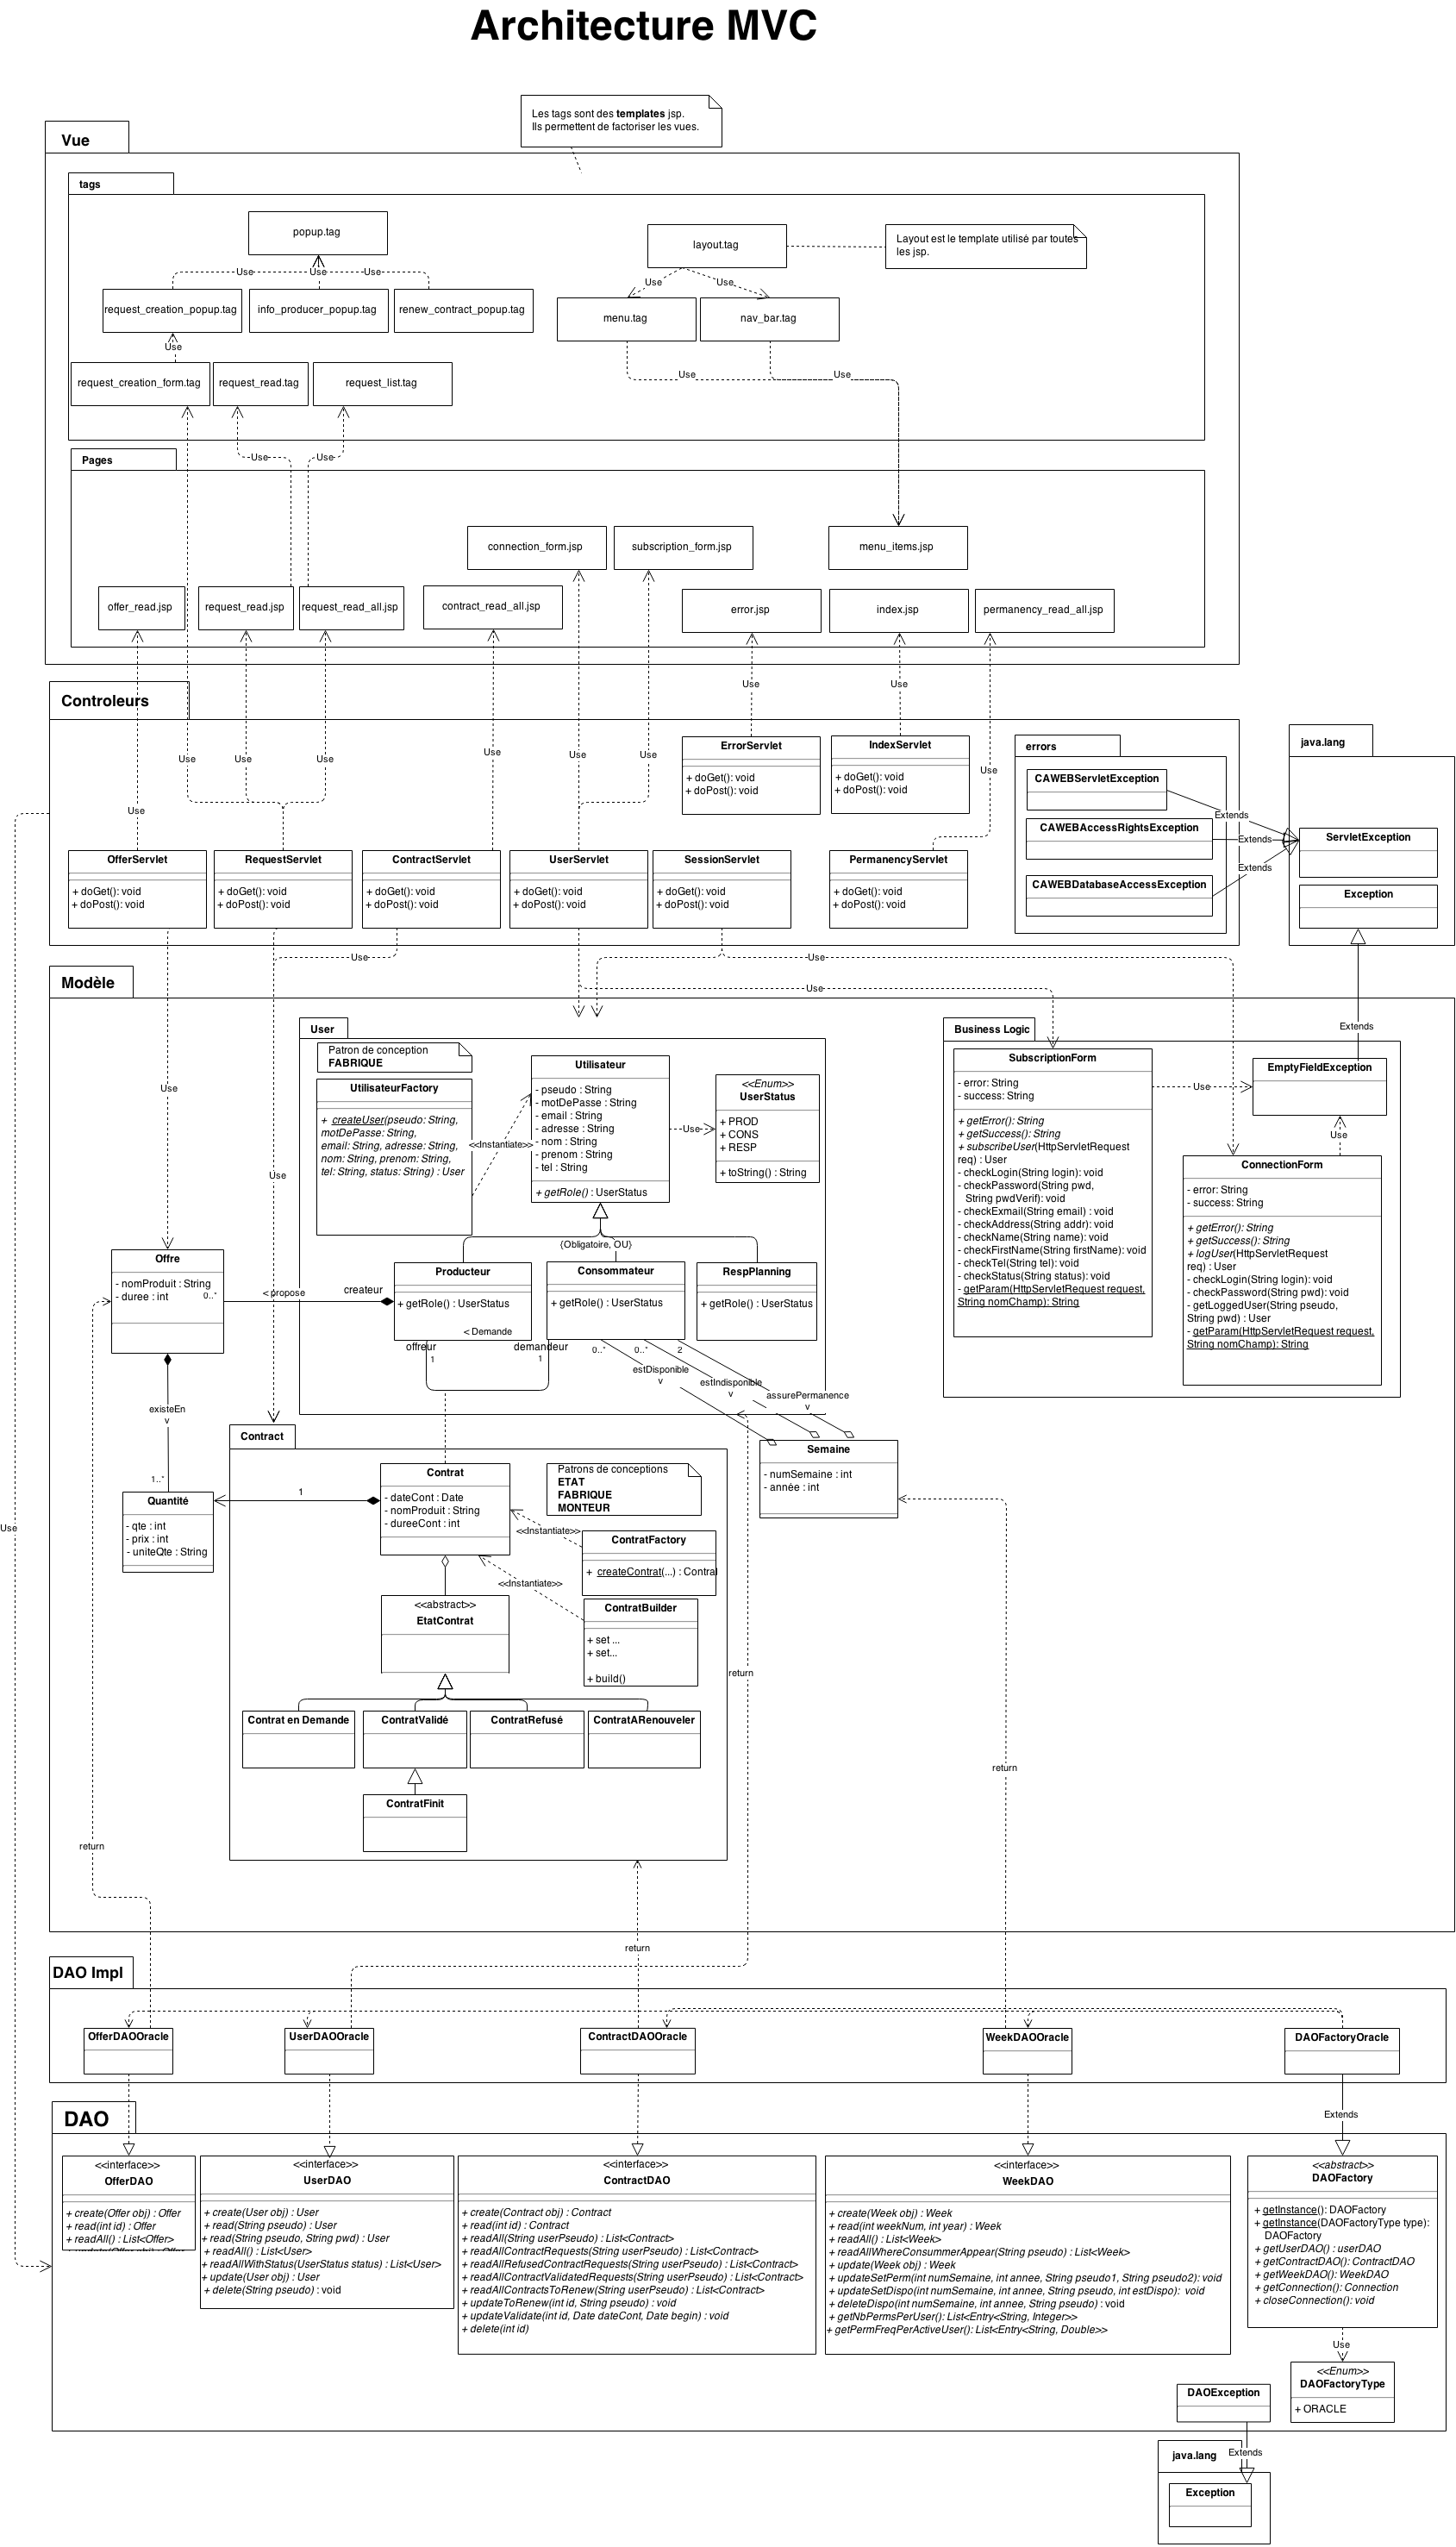
\includegraphics[height=1.1\textwidth]{./ressources/architecture.png}
\caption{Architecture logicielle.}
\end{figure}
\clearpage


\begin{figure}[!hp]
\centering
\subsection{Diagramme de classes logicielles~~~~~~~~~~~~~~~~~~~~~~~~~~~~~~~}
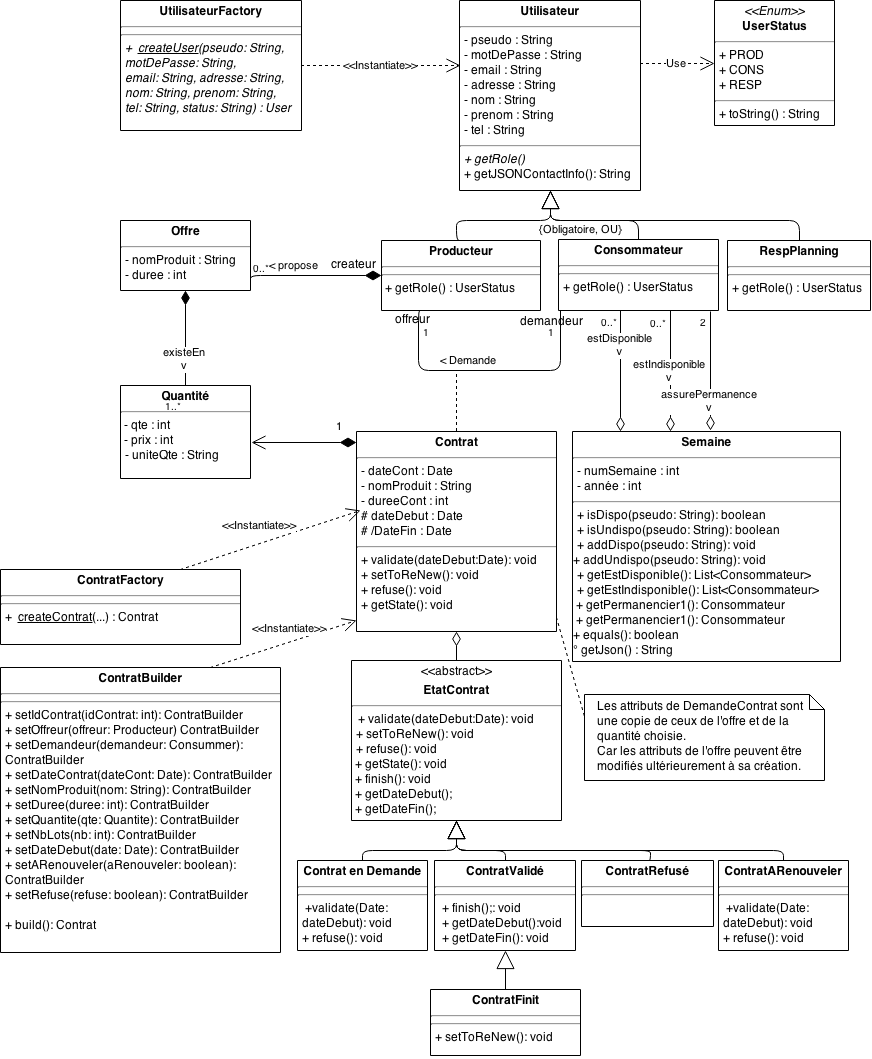
\includegraphics[height=1.\textwidth]{./ressources/class_logicielle.png}
\caption{Diagramme de classes logicielle.}
\end{figure}
\clearpage

\subsection{Diagrammes de séquence}
TODO

\subsection{Diagrammes d'états-transitions}
TODO
\begin{figure}[!hp]
\centering
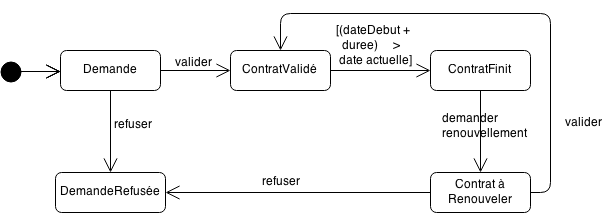
\includegraphics[width=1.\textwidth]{./ressources/etat_transition_contrat.png}
\caption{Cycle de vie d'un contrat}
\end{figure}
\clearpage

\section{Manuel Utilisateur}
TODO

\section{Bilan sur les outils de modélisation}
Afin de réaliser nos différents diagrammes, nous avons utilisé l'application web \textit{Draw.io Pro} \footnote{Draw.io : \url{www.draw.io}}.\\
Nous n'avons pas rencontré de difficulté particulière à ce niveau. Les formes "UML" et "SysML" disponibles dans \textit{Draw.io} permettent de réaliser l'ensemble des diagrammes de la norme UML2.


\end{document}